\documentclass[sigconf]{acmart}
\usepackage{subcaption}

% Copyright
%\setcopyright{none}
%\setcopyright{acmcopyright}
%\setcopyright{acmlicensed}
\setcopyright{rightsretained}
%\setcopyright{usgov}
%\setcopyright{usgovmixed}
%\setcopyright{cagov}
%\setcopyright{cagovmixed}


% DOI
\acmDOI{To_be_inserted_after_paper_is_accepted}

% ISBN
\acmISBN{000-0000-00-000/00/00}

%Conference
\acmConference[AIR 2017]{Advances in Robotics}{June 28-July 02, 2017}{New Delhi, India}
\acmYear{2017}
\copyrightyear{2017}

\acmPrice{15.00}


\begin{document}
\title{Robotic cloth manipulation for clothing assistance task using Dynamic Movement
Primitives}
\titlenote{Produces the permission block, and copyright information}
%\subtitle{Extended Abstract}
%\subtitlenote{The full version of the author's guide is available as
%  \texttt{acmart.pdf} document}


\author{Ravi P. Joshi}
\authornote{Dr.~Trovato insisted his name be first.}
\orcid{1234-5678-9012}
\affiliation{%
	\institution{Institute for Clarity in Documentation}
	\streetaddress{P.O. Box 1212}
	\city{Dublin}
	\state{Ohio}
	\postcode{43017-6221}
}
\email{joshi-ravi-prakash@edu.brain.kyutech.ac.jp}

\author{Nishanth Koganti}
\authornote{The secretary disavows any knowledge of this author's actions.}
\affiliation{%
	\institution{Institute for Clarity in Documentation}
	\streetaddress{P.O. Box 1212}
	\city{Dublin}
	\state{Ohio}
	\postcode{43017-6221}
}
\email{nishanth-k@is.naist.jp}

\author{Tomohiro Shibata}
\authornote{This author is the
one who did all the really hard work.}
\affiliation{%
	\institution{The Th{\o}rv{\"a}ld Group}
	\streetaddress{1 Th{\o}rv{\"a}ld Circle}
	\city{Hekla}
	\country{Iceland}}
\email{tom@brain.kyutech.ac.jp}

% images are stored inside images directory
\graphicspath{{./images/}}

\begin{abstract}
	The need of robotic clothing assistance in the field of assistive robotics is growing, as it is one of the most basic activities in daily life of elderly and disabled people. In this study, we are investigating the applicability of using Dynamic Movement Primitives (DMP) as a task parameterization model for performing clothing assistance tasks. The robotic cloth manipulation task deals with putting the cloth on both the arms. The clothing assistance is a challenging problem since robot must do cooperative manipulation by holding the cloth using both the arms while interacting with non-rigid and highly deformable clothes, and with the assisted person whose posture can vary during the assistance. The system consists of dual arm Baxter research robot and Microsoft Kinect V2 RGBD sensor for tracking the posture of arms. The cloth manipulation is done by Baxter robot which follows the trajectory generated by DMP system. We have performed the experiments on soft mannequin instead of human. The result shows that DMPs are able to generalize the movement trajectory for the modified posture.
\end{abstract}

%
% The code below should be generated by the tool at
% http://dl.acm.org/ccs.cfm
% Please copy and paste the code instead of the example below.
%
\begin{CCSXML}
	<ccs2012>
	<concept>
	<concept_id>10010520.10010553.10010562</concept_id>
	<concept_desc>Computer systems organization~Embedded systems</concept_desc>
	<concept_significance>500</concept_significance>
	</concept>
	<concept>
	<concept_id>10010520.10010575.10010755</concept_id>
	<concept_desc>Computer systems organization~Redundancy</concept_desc>
	<concept_significance>300</concept_significance>
	</concept>
	<concept>
	<concept_id>10010520.10010553.10010554</concept_id>
	<concept_desc>Computer systems organization~Robotics</concept_desc>
	<concept_significance>100</concept_significance>
	</concept>
	<concept>
	<concept_id>10003033.10003083.10003095</concept_id>
	<concept_desc>Networks~Network reliability</concept_desc>
	<concept_significance>100</concept_significance>
	</concept>
	</ccs2012>
\end{CCSXML}

\ccsdesc[500]{Computer systems organization~Embedded systems}
\ccsdesc[300]{Computer systems organization~Redundancy}
\ccsdesc{Computer systems organization~Robotics}
\ccsdesc[100]{Networks~Network reliability}

% We no longer use \terms command
%\terms{Theory}

\keywords{Robotic Clothing Assistance, Dynamic Movement Primitives (DMP), Human-Robot Interaction, Learning and Adaptive Systems}


\maketitle

\begin{figure}
	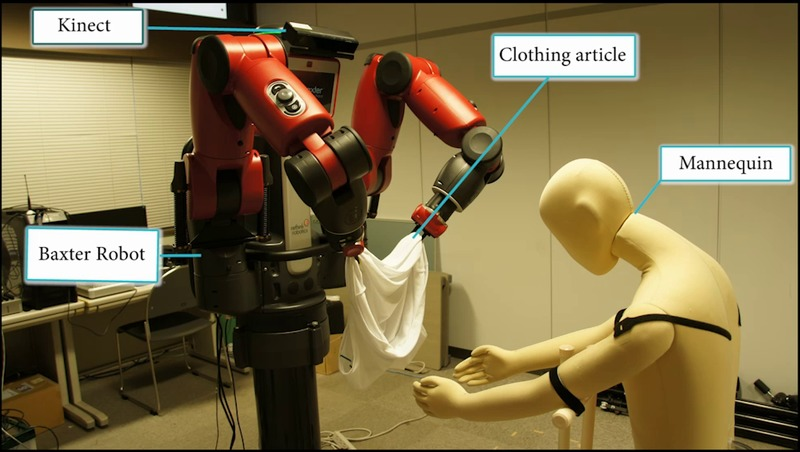
\includegraphics[width=\linewidth]{setup}
	\caption{Setup of Robotic cloth manipulation task}
	\label{fig:setup}
\end{figure}

\section{Introduction}
\label{sec:introduction}
Due to the demographic trend in developed countries, the robotic assistance in the field of elderly care in home environment is growing \cite{broekens2009assistive}. Although there has been a significant number of research done in this field, the robotic clothing assistance is yet an open field for research. Not to mention that, it is one of the basic and important assistance activities in daily life of elderly as well as disabled people. While rigid object manipulation with robots has mainly relied on precise robot control, the deformable objects rather require complex control scheme. The clothing assistance is a challenging problem since robot is required to manage two difficulties: (a) robot must do cooperative manipulation by holding the cloth using both the arms while interacting with non-rigid and highly deformable clothes and (b) maintain safe human-robot interaction with the assisted person whose posture can vary during the assistance.

In this study, we are investigating the applicability of using Dynamic Movement Primitives (DMP) as a task parameterization model for performing clothing assistance tasks. The robotic cloth manipulation task deals with putting the cloth on both the arms. The idea of using DMP is inspired from the fact that DMP can learn complex task from the demonstration \cite{ijspeert2003learning, schaal2006dynamic, ijspeert2013dynamical} and thus reduce the manual efforts to design the controller from scratch or to fine-tune the controller parameters. We choose the dual arm Baxter robot in this research as it is safe and flexible by design \cite{fitzgerald2013developing}.

The rest of the paper is organized as follows. Section \ref{sec:related_works}, gives a brief overview about the related literature in this field. Section \ref{sec:dmp} introduces the mathematical formulation about Dynamic Movement Primitives. In Section \ref{sec:system_overview}, we describe our system and various components used in the experiments. Section \ref{sec:experiments} deals with the details about experiments performed. Section \ref{sec:results} shows the experimental results. Finally we conclude in Section \ref{sec:conclusions} with some future directions.

\section{Related Works}
\label{sec:related_works}
In this section, we provide brief overview of the related literature in this field. There has been significant number of research done in the field of Robotic Clothing Assistance. Colom{\'e} et al. \cite{colome2015friction} proposed a framework for Reinforcement Learning of robotic tasks in non-rigid environments. They performed the task of wrapping a scarf around the neck of a mannequin and used color based segmentation to distinguish mannequin, scarf and a mark placed on the nose of mannequin. The main focus of their work is to incorporate friction based model while performing clothing task. Gao et al. \cite{gao2015user, gao2016iterative} has focused on user upper-body modeling for personalized dressing by using top-view depth camera. Randomised decision forests was used to estimate user pose and proposed an online iterative path optimisation method to enable Baxter humanoid robot to assist human to wear a sleeveless jacket. Another interesting work by Kapusta et al. \cite{kapusta2016data} is focused towards designing a controller inspired from data-driven haptic perception. They classified the forces measured at robot's end effector by using hidden Markov models and performed the clothing task on hospital gown. Their focus was to classify force data for haptic perception with high accuracy. Klee et al. \cite{klee2015personalized} worked on personalized assistance for dressing a user, where they used vision module to monitor the human's motion. The robot request to user to move towards robot, monitors motion and puts hat on the user once users is rechable by the robot. Koganti et al. \cite{koganti2015cloth} proposed a framework for offline learning of cloth dynamics model using Gaussian Process Latent Variable Models (GP-LVM) by incorporating motion capture data and applying this model for the online tracking of human-cloth relationship using a depth sensor. They showed that the shared GP-LVM is able to learn reliable motion models of the T-shirt state for robotic clothing assistance tasks. Representing cloth state in low-dimensional field by using topology coordinates is another impressive work done by Tamei et al. \cite{tamei2011reinforcement}. They proposed Reinforcement Learning framework and demonstrated that the robot quickly learns a suitable arm motion for putting T-shirt into the mannequin's head. Yamazaki et al. \cite{yamazaki2013method, yamazaki2014bottom}  worked on bottom dressing by a life-sized humanoid robot, where they recognize the cloth state by using  optical flow on the images acquired from single camera. They showed that the robot can pull a bottom clothing item along the subject's legs.

Another related filed of research is motor-skills learning for Cloth Handling, in which Yamakawa et al. \cite{yamakawa2011dynamic} proposed a new strategy for dynamic manipulation of sheet-like flexible objects by a high-speed robot system. The system consists of two high-speed multi-fingered hands mounted on two sliders and a high-speed vision system. The proposed system learns the necessary motor skills from the demonstration performed by a human subject. They validated the robot trajectory obtained from the motion planning method was with simulation results. Another exciting work done by Mons{\'o} et al. \cite{monso2012pomdp}, where they proposed a probabilistic planner, based on Partially Observable Markov Decision Process (POMDP) approach, for reducing the inherent uncertainty of cloth sorting (isolation/extraction) task. Their approach relaxes the precision requirements of robot vision and manipulation.

\begin{figure}
	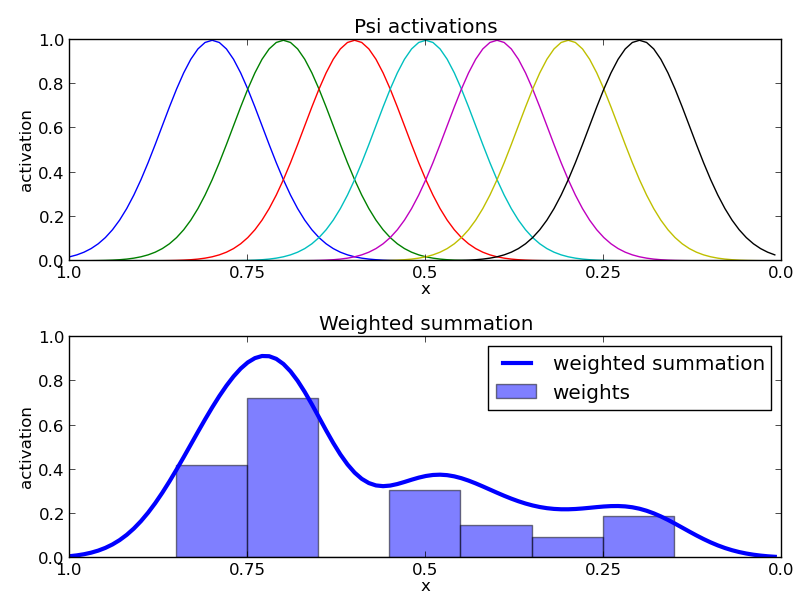
\includegraphics[width=\linewidth]{psi}
	\caption{$\psi$ activations and weighted summation of Gaussians}
	\label{fig:psi_activations}
\end{figure}

\section{Dynamic Movement Primitives}
\label{sec:dmp}
Dynamic Movement Primitives (DMP) aims at designing contoller for learning and generalization of motor skills by learning from demonstration \cite{ijspeert2003learning}. The controllers are based on nonlinear dynamical systems, and use locally weighted regression techniques to learn complex, discrete or rhythmic, movements demonstrated by a human subject \cite{ijspeert2002movement}. These controllers can be considered to be discrete or rhythmic pattern generators which can replay and modulate the learned movements, while being robust against perturbations.

The basic idea behind DMP formulation is to use an analytically well-understood dynamical system and add a nonlinear terms, so that it produces the desired behavior \cite{ijspeert2013dynamical}. Formally, the system is defined by a damped spring model as below:

\begin{equation}
	\tau	 \dot{v} = K (g - x) -D v - K (g - x_0) s + K f(s)
\end{equation}
\begin{equation}
	\tau	 \dot{x} = v
\end{equation}

The term $x$ and $v$ are position and velocity of the system respectively, $x_0$ and $g$ are start and goal position, $\tau$ is a scaling term, $K$ is spring constant and $D$ is damping factor. The nonlinear function $f$, which is also called as forcing term is a non-linear function to be learned to allow complex movements. The forcing function $f$ is chosen as

\begin{equation}
	f(s) = \frac{\Sigma_{i} w_i \psi_i(s)}{\Sigma_{i} \psi_i(s)} s
	\label{eq:forcing_func}
\end{equation}

where $\psi_i$ is defined as Gaussian basis function as
\begin{equation}
	\psi_i = \textrm{exp}\left( -h_i \left( s - c_i\right)^2 \right)
\end{equation}

where $h_i$ and $c_i$ are constants that determine, respectively, the width and centers of the basis functions. $w_i$ represents the weight defined for each Gaussian. The forcing function $f$ depends on phase variable $s$. Phase variable $s$ starts from 1 and monotonically decreases to 0, defined by equation below:

\begin{equation}
	\tau \dot{s} = - \alpha s
\end{equation}

where $\alpha$ is a positive gain term. Our goal is to design the forcing function that can learn from the demonstration and allows us to scale the movement defined by goal state $g$. In other words, we want to setup the system which can follow a specified path. The forcing term can be redefined as:

\begin{equation}
	f_{target}(s) = \frac{D v + \tau \dot{v}}{K} - - (g - x) +  (g - x_0) s
\end{equation}

where desired acceleration $\dot{v}(t)$ can be calculated by double differentiating the position data recorded from the demonstration as

\begin{equation}
	\dot{v}(t) = \frac{\partial}{\partial t} v(t) = \frac{\partial}{\partial t} \frac{\partial}{\partial t} x(t)
\end{equation}

The forcing function [\ref{eq:forcing_func}] is comprised of weighted summation of Gaussian that are going to be activated as system converges to the goal as shown in figure \ref{fig:psi_activations}. We want that forcing function matches the desired trajectory. In other words, we want $f_{target}$ to be as close as possible of $f$ as written below:

\begin{equation}
	J = \sum_{s} \left( f_{target}(s) - f(s) \right)^2
\end{equation}

This ends by calculating the weight parameters across Gaussians. Optimization methods such as locally weighted regression \cite{vijayakumar2000locally} can be used, so that the forcing function matches the desired trajectory. This way DMP can be made to imitate the desired path \cite{pastor2009learning}.

\section{Overview of the System}
\label{sec:system_overview}
Robotic cloth manipulation task contains a dual arm humanoid robot Baxter. Setup of the system is shown in figure \ref{fig:setup}. We choose soft mannequin instead of a human for this preliminary experiment. Both the arms of mannequin are open and  given the support by a metallic stand, to avoid falling down the arms. The mannequin is positioned in such a way, so that it resides within the limits of work space of the Baxter robot. Both the arms of mannequin are facing towards robot. A Kinect V2 \cite{microsoft2014kinect} sensor is mounted on LCD display of Baxter root. Kinect sensor can see the mannequin and clothing article and provides depth information, which is necessary for mannequin tracking. The clothing article is put in arms of Baxter robot manually before starting the experiment.

The Baxter robot is connected to a computer directly using Ethernet cable. It is controlled using Robot Operating System (ROS) \cite{quigley2009ros}, one of the widely used tool by the researchers in robotics community. We used Baxter robot's API, which are available and supported by ROS to command the robot. The Kinect sensor is controlled by Open source Kinect API for ROS \cite{iai_kinect2, libfreenect2}.

\begin{figure*}
	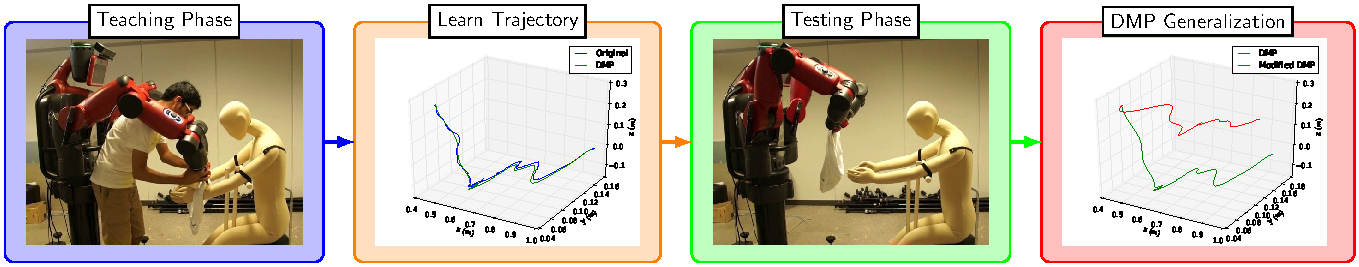
\includegraphics[width=\linewidth]{flowchart_conf}
	\caption{Work flow of Robotic cloth manipulation task. Initially a demonstration is performed by moving the Baxter arms in the appropriate trajectory. The demonstration is recorded and parameterized by DMP. Later posture of the mannequin is changed and accordingly the goal posture of DMP is modified. Now, the modified DMP can accommodate new posture.}
	\label{fig:workflow}
\end{figure*}

\section{Experiments}
\label{sec:experiments}
As per the formulation described in section \ref{sec:dmp}, DMP can learn by the demonstration. Therefore we start by performing a demonstration by holding the robot arm and move accordingly. During the demonstration, pose of the end-effector is recorded. The term pose collectively refers to position and orientation. Once the demonstration is finished, DMP is initialized using the recorded trajectory. Three DMP trajectories one for each coordinate axis are initialized for one arm. In this way, we have totally six DMP trajectories, which can control both the arms of Baxter robot. We performed following two experiments by using these trajectory: (a) Clothing task using position DMP (b) Failure detection using end-effector forces.

\subsection{Clothing task using position DMP}
The aim of this experiment is to put the clothing article on both the arms of mannequin by using DMP system. We use the position data to initialize the DMP trajectories, which are being used in this task. The posture of mannequin is changed by lifting the arms up or down. At this point, we use Kinect Sensor to get the 3D coordinates of the arm. Now we change the goal of DMP trajectories by using this information. The modified DMP can be acquired as described in section \ref{sec:dmp}.

\subsection{Failure detection using end-effector forces}
This experiment is designed to deal with failure cases. There can be many failure cases during the clothing task, such as the clothing article gets stuck into the fingers. In this experiment, we are using forces being applied on the end-effector of Baxter robot to detect the failure scenario. Appropriate action can be taken once the failure is detected.

\section{Results}
\label{sec:results}
A soft mannequin was used in order to perform the clothing task. A sleeveless T-shirt was used during the experiment and the task was to put the clothing article on both the arms as shown in figure \ref{fig:various_posture}. Following subsections explains the results of the two experiments described above.

\begin{figure}
	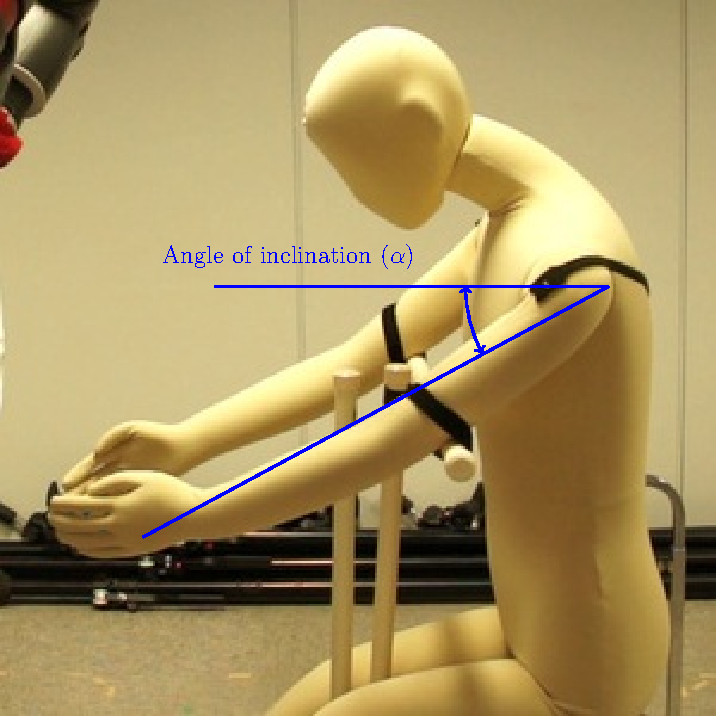
\includegraphics[width=\linewidth]{inclination}
	\caption{Angle of Inclination}
	\label{fig:inclination}
\end{figure}

\begin{figure}
	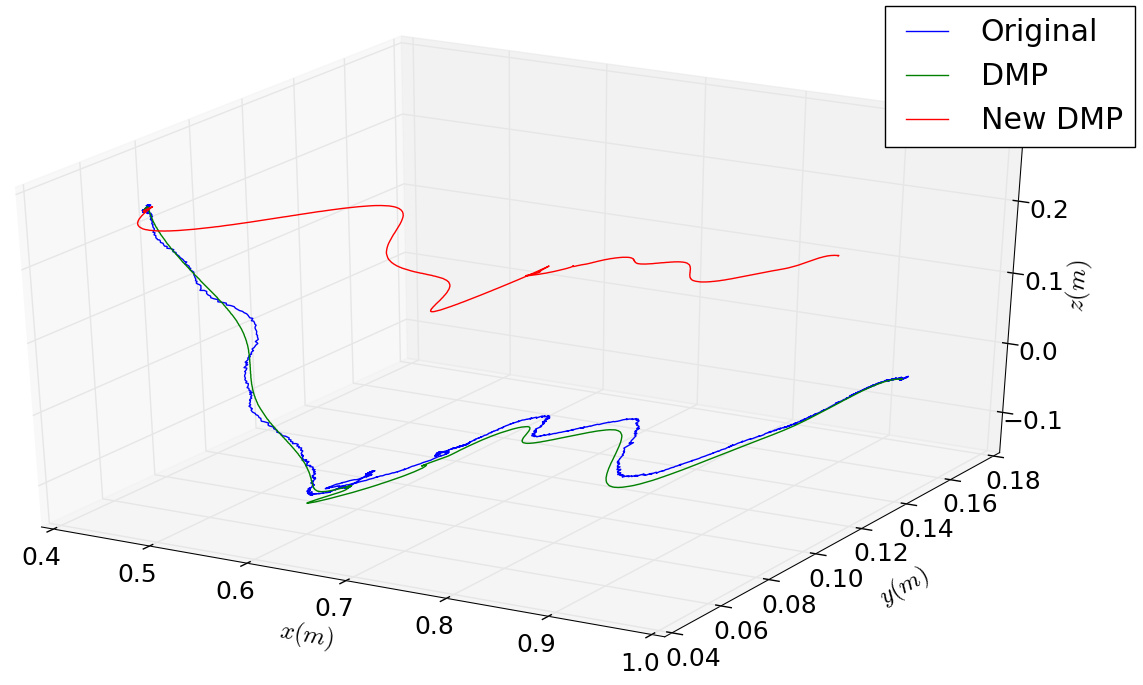
\includegraphics[width=\linewidth]{trajectory}
	\caption{Left arm trajectory of Baxter}
	\label{fig:trajectory}
\end{figure}

\subsection{Clothing task using position DMP}
In this experiment, the initialized DMP was modified to accommodate the new posture by changing the goal state of the DMP. The generated trajectory was then run on the Baxter robot as shown in figure \ref{fig:trajectory}. The newly generated DMP trajectory (shown in red color) was not only found well suited and capable of performing clothing task but also smooth compared to the original trajectory (shown in blue color). A video demonstartion of this experiment can be seen at YouTube\footnote{\url{http://youtu.be/Rb2JePazJjk}}.

To eventuate this experiment, we performed it many times for various postures by keeping the arms at different-different height. During the experiment, we monitored the trajectory generated by DMP system. The accuracy measurement is shown in figure \ref{fig:accuracy}.

\begin{figure}
	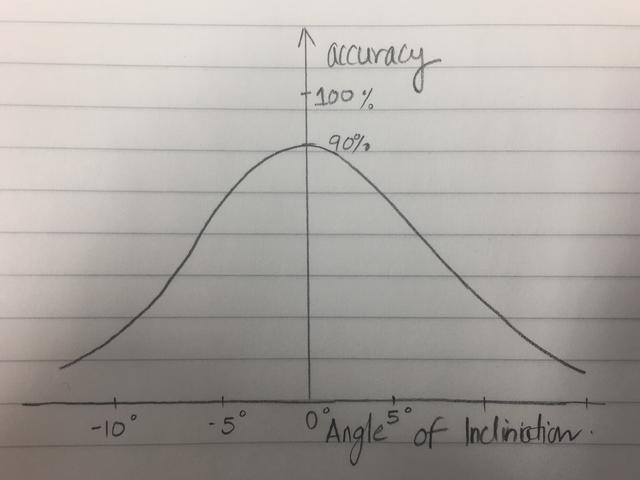
\includegraphics[width=\linewidth]{accuracy}
	\caption{Accuracy measurement}
	\label{fig:accuracy}
\end{figure}

\subsection{Failure detection using end-effector forces}
The clothing task has to deal with complex dynamics including manipulation of clothing article. The clothes are non-rigid, flexible and highly deformable objects, making the task more difficult to perform. During the clothing task, we observed the forces being applied at both the end-effector of Baxter robot. The trajectories were monitored and categorized into two \textit{success} and \textit{failure}. The mean of these two category is calculated and plotted as shown in figure \ref{fig:position_force}.

It is clearly visible from the figure \ref{fig:position_force} that the applied forces are very different in nature in both the cases. Both of these applied forces are increasing from the beginning however the applied forces in case of \textit{failure} are much more higher than that of \textit{success}. Hence one can easily differentiate and detect the failure by using this information.

\begin{figure}
	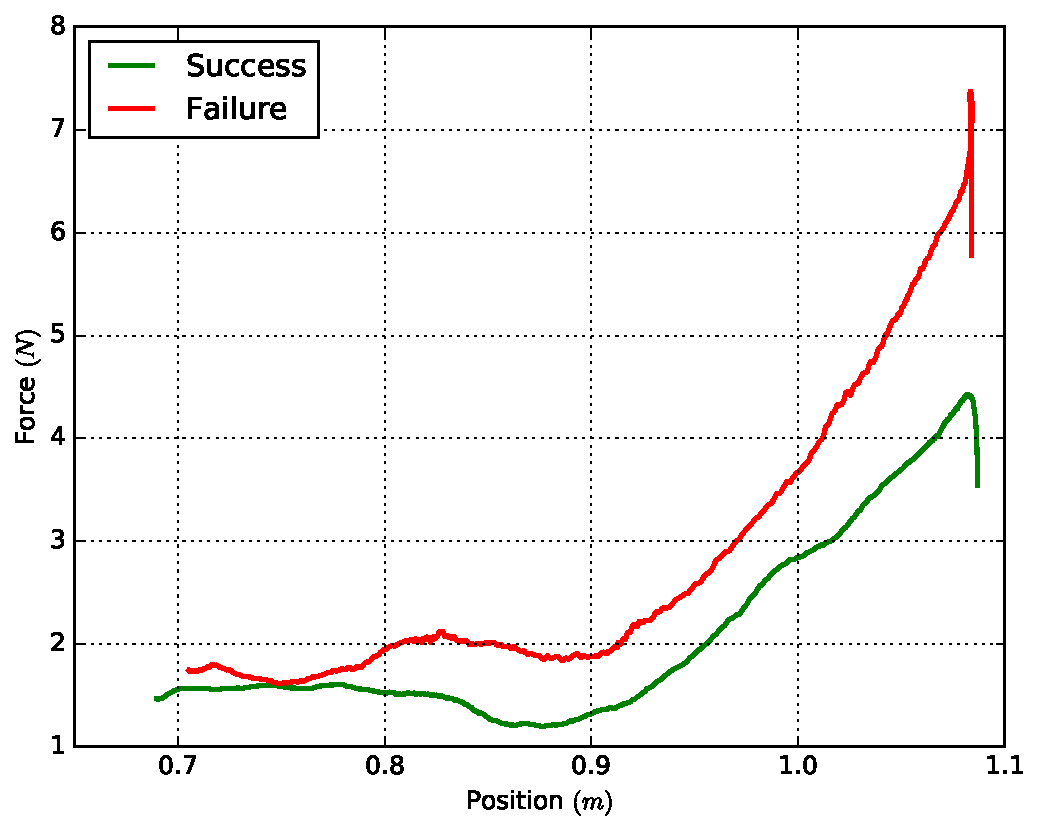
\includegraphics[width=\linewidth]{position_force}
	\caption{Failure detection using end-effector forces}
	\label{fig:position_force}
\end{figure}

\section{Conclusions}
\label{sec:conclusions}
This paper presents an approach for robotic cloth manipulation for clothing assistance task using Dynamic Movement Primitives. A dual arm Baxter robot, soft mannequin and very thin sleeveless T-shirt were used in the task. We have also presented an approach for failure detection using forces being applied on the end-effector of the robot. We have used the Baxter APIs in order to get the forces, which are calculated by Baxter Dynamics Module. Though raw forces were very noisy in nature, but after applying median filter most of the noise was eliminated properly.

We plan to extend our research to make the approach more robust by adding visual information and force information with DMP system in the future. Also there is a need of designing an adaptive controller for real time tracking to adapt and detect various failure scenarios. Therefore, in the future, a combination of robot vision and force data can provide the better estimation of cloth state.

\begin{acks}
	The authors would also like to thank the anonymous referees for their valuable comments and helpful suggestions. The work is supported by the \grantsponsor{GS501100001809}{National Natural Science Foundation of China}{http://dx.doi.org/10.13039/501100001809} under Grant No.:~\grantnum{GS501100001809}{61273304} and~\grantnum[http://www.nnsf.cn/youngscientsts]{GS501100001809}{Young Scientsts' Support Program}.
\end{acks}

\bibliographystyle{ACM-Reference-Format}
%\bibliographystyle{unsrt}
\bibliography{air}

\end{document}
